\chapter{Design and Implementation}
\label{chap:implementation}


\section{Feature summary}
This project has successfully built and deployed \textcolor{NavyBlue}{\textsc{Solbolt}}, a compiler explorer and gas analysis tool,
which is available for all to use on the live website at \href{https://www.solbolt.com}{\textcolor{NavyBlue}{solbolt.com}} \cite{solbolt}. Next, we shall examine some of its
key features, with reference to a summary graphic shown in Figure \ref{fig:solbolt_summary}.

\subsection{Solidity Compilation}

\begin{sidewaysfigure}
  \centering
  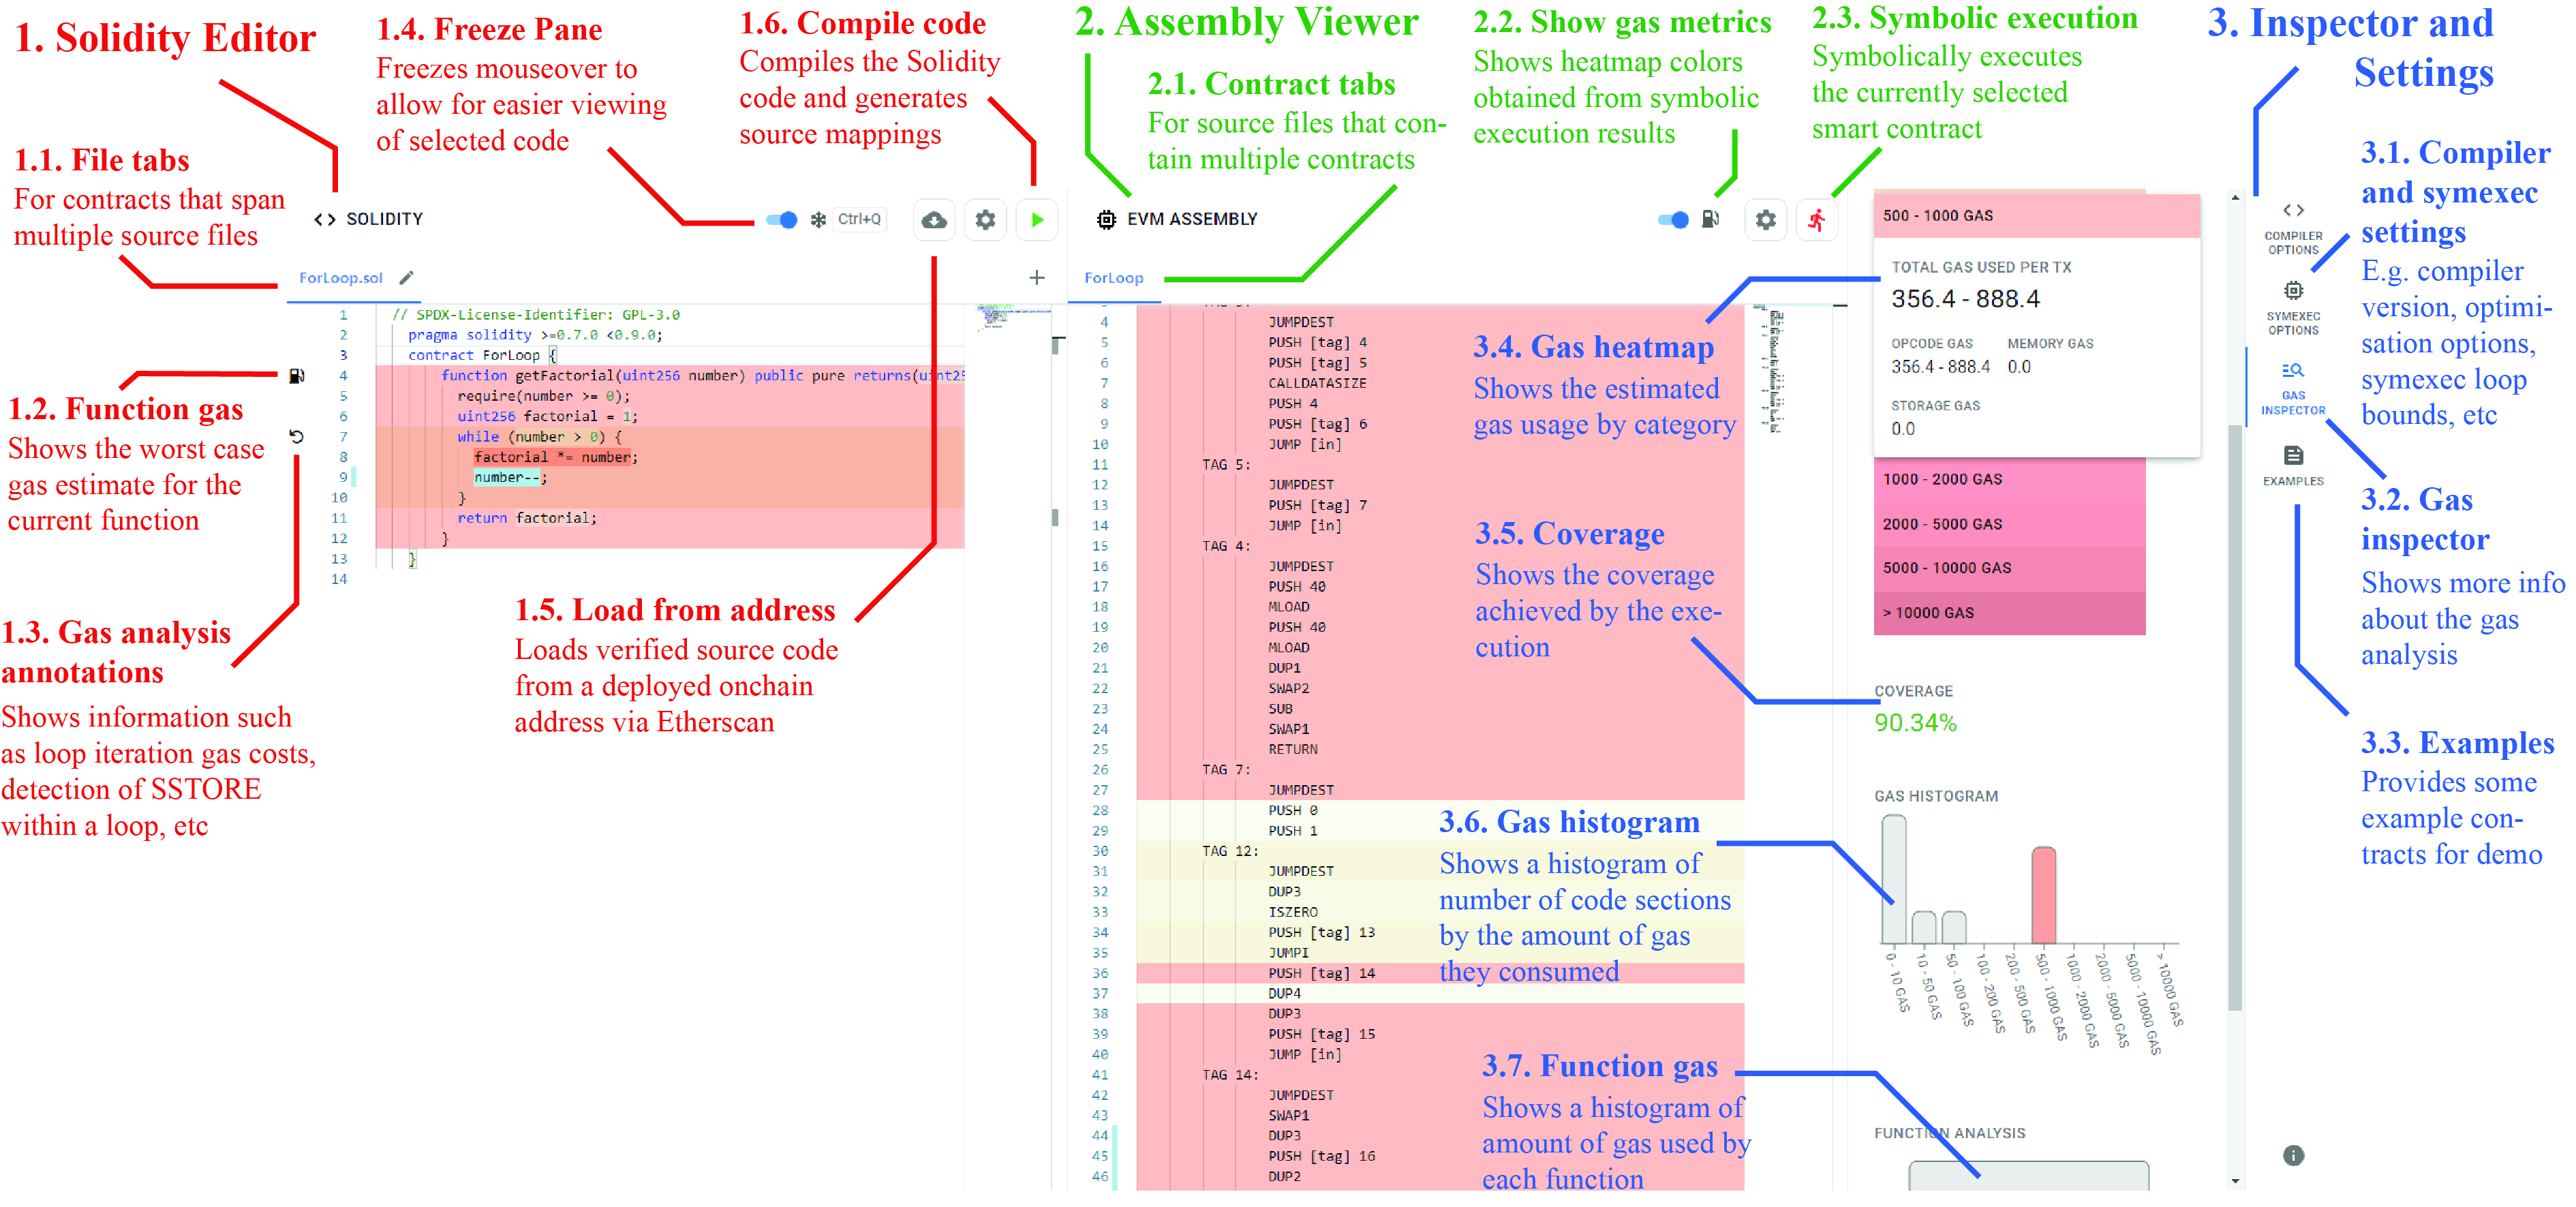
\includegraphics[width=\textwidth]{./figures/implementation/summary}
  \caption{Summary of \textcolor{NavyBlue}{\textsc{Solbolt}} features}
  \label{fig:solbolt_summary}
\end{sidewaysfigure}

The tool supports the compilation of contracts written in Solidity version 0.4.17 to 0.8.13,
as well as support for EVM version from \texttt{homestead} to \texttt{berlin}. This is, to
our knowledge, the most up-to-date and widest available compiler support for any 
Solidity gas analysis tool so far. The user also has the option to enable optimisation, as
well as customise advanced options such as enabling the peephole optimiser, the inliner,
the common subexpression eliminator, and more, as seen in Figure \ref{fig:solbolt_compiler_options}. This may be helpful for developers or
researchers investigating the effects of different optimisation options.

The tool also supports the compilation of contracts spread over multiple source files,
as well as compiling multiple contracts from the same source. For verified contracts that
are already deployed on chain, the tool also has Etherscan integration, and can directly
load a contract from a verified Ethereum address for compilation, using Item 1.5 
as indicated in the summary graphic.

After successful compilation of the source, the EVM assembly opcodes will be displayed
on the right ``Assembly viewer" pane. Sections of the opcodes will be colour-coded based 
on its mapping to the Solidity source code, similar to the Godbolt tool that inspired this
project. Hovering over a section will also highlight and bring to view its corresponding
mapped section on the other pane, which can be frozen via a keyboard shortcut.

\begin{figure}[h]
  \centering
  \subfloat[\centering Compiler options]{{\label{fig:solbolt_compiler_options}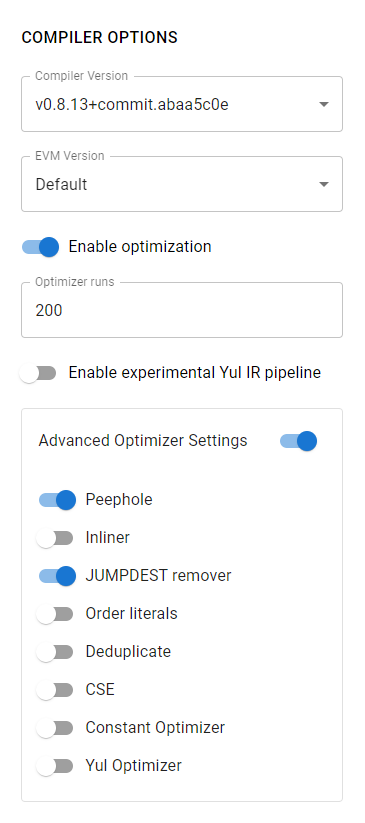
\includegraphics[width=0.3\textwidth]{./figures/implementation/compiler_options} }}%
  \qquad
  \subfloat[\centering Symbolic execution options]{{\label{fig:solbolt_symexec_options}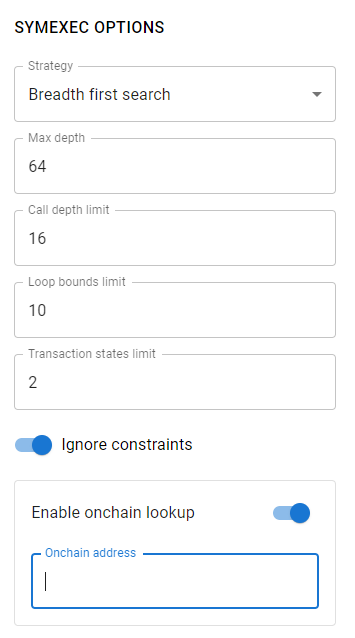
\includegraphics[width=0.3\textwidth]{./figures/implementation/symexec_options} }}%
  \caption{\textcolor{NavyBlue}{\textsc{Solbolt}} options}%
  \label{fig:solbolt_options}%
\end{figure}


\subsection{Symbolic Execution}

Once the source is compiled, users are able to run a symbolic execution using Item 2.3.
The symbolic execution instance will try to execute each path of the contract bytecode,
and derive gas estimates for each mapping generated by the compiler. This is indicated to
the user as a coloured heatmap for quick identification of the gas-costly sections, 
with lighter yellow shades consuming fewer gas units,
while the darker red shades consuming greater gas units. 

Next, it will also calculate worst case gas estimates for each function it detects, as 
well as per-iteration gas costs for
each loop, including hidden loops within compiler generated code. Finally, the
symbolic executor can also detect common gas inefficient patterns, such as modifying a 
storage variable within a loop, which could possibly be fixed or refactored for 
additional gas savings.

Each symbolic execution is run with a timeout of 120 seconds, and users can customise
some of its settings, such as the path traversal strategy, the maximum depth, 
the call depth limit, the loop bounds limit, and the number of transactions to run, 
as seen in Figure \ref{fig:solbolt_symexec_options}. 

This
may be important to tweak for different contracts to achieve the best results,
depending on how complex they are, how many times a loop is expected to run, and so on.
The user can also enable the Z3 SMT solver, which prunes paths that are not reachable as
the constraints placed on them are not satisfiable. 
Users can also provide a on chain address for symbolic execution, 
and the engine will make use of the live concrete storage state of that address instead of
a symbolic storage state.

\subsection{Gas Inspector}

Finally, the user is able to refer to the gas inspector tab on the right for a more detailed
gas analysis report, as indicated
by Item 3. Here, there is a gas heatmap legend indicating the total estimated gas used
per transaction by the code section that is currently highlighted, 
as well as the gas used by the different categories, as seen with Item 3.4.
It also shows the coverage percentage achieved by the symbolic execution, shown with Item 3.5. 

The gas histogram,
as seen with Item 3.6, shows a gas profile of the smart contract by plotting the total number
of code sections that fall under a certain gas usage class. Lastly, Item 3.7 shows a histogram
of worst case gas usage by each executed function.

\clearpage
\section{Architecture Design}

\begin{figure}[h]
  \centering
  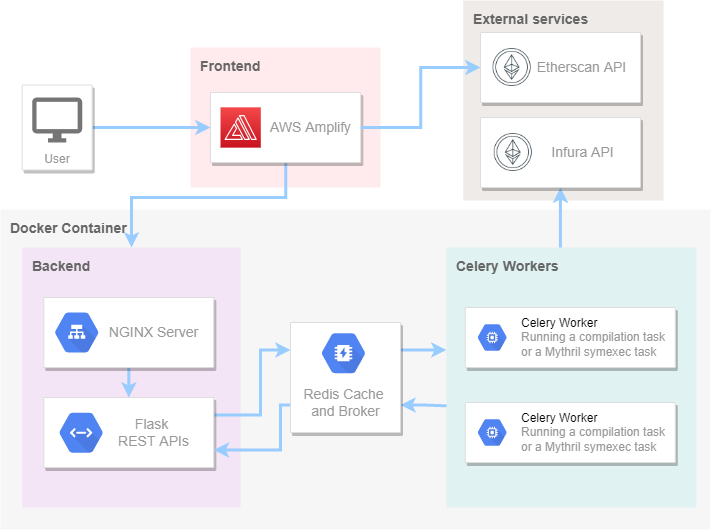
\includegraphics[width=0.8\textwidth]{./figures/implementation/architecture}
  \caption{\textcolor{NavyBlue}{\textsc{Solbolt}} architecture overview}
  \label{fig:solbolt_architecture}
\end{figure}

\subsection{UI Elements and Redux State Management}
The \textcolor{NavyBlue}{\textsc{Solbolt}} frontend is built from scratch using React (Typescript) 17.0.2 and Material UI 5.3.1.
It is designed as a Single-Page Application (SPA), with three main panels for simple
simple navigation, as seen in the screenshot in Figure \ref{fig:solbolt_summary}.
We chose to develop \textcolor{NavyBlue}{\textsc{Solbolt}} fully in Typescript rather than Javascript, because although
this required the definition of additional interfaces and typing of arguments, it also
provided benefits such as code hints and error highlighting when the expected types of objects
did not match.

A common challenge we faced when designing the frontend was having to pass and manage props
deeply into nested components when using React.
This was addressed by making extensive use of redux, \texttt{useContext} and hooks.
For example, for managing the contract state, we created an \texttt{ContractsContext} that
included the \texttt{ContractsState}, as well as functions to update the 
\texttt{ContractsState}, as seen in Listing \ref{lst:solbolt_contracts_context}.


\begin{lstlisting}[language=Javascript, caption={\texttt{ContractsContext} used for managing contract state}, label={lst:solbolt_contracts_context}, basicstyle=\ttfamily\scriptsize]
  const ContractsContext = 
    createContext<
      [ContractsState | undefined, {
        updateContract: 
          ((filename: string, name: string, contract: ContractJSON) => void) | undefined, 
        updateAllContracts: 
          ((contracts: {[fileName: string]: {[contractName: string]: ContractJSON}}, 
            ast: {[name: string]: any}) => void) | undefined
      }]
    >([undefined, {
          updateContract: undefined, 
          updateAllContracts: undefined
      }]);
\end{lstlisting}

\texttt{ContractsContext} also has a \texttt{reducer}, which takes an update type and a payload.
Depending on the type of the update, the \texttt{reducer} will modify the state accordingly,
making use of relevant data in the payload, as seen in Listing \ref{lst:solbolt_contracts_reducer}

\begin{lstlisting}[language=Javascript, caption={Reducer used in \texttt{ContractsContext}}, label={lst:solbolt_contracts_reducer}, basicstyle=\ttfamily\scriptsize]
  function reducer(state: ContractsState, { type, payload }: { type: UpdateTypes, payload: PayloadType | undefined}) {
    switch (type) {
      case UpdateTypes.UPDATE_CONTRACT: {
        /* Perform update for one contract */
        ...
      }

      case UpdateTypes.UPDATE_ALL_CONTRACTS: {
        /* Perform update for ALL contracts */
        ...
      }

      default: {
        throw Error(`Unexpected action type in ContractsContext reducer: '${type}'.`)
      }
    }
  }
\end{lstlisting}

This \texttt{reducer} is called by the \texttt{Provider}, which lives near the root of
the React DOM, above all of the components that wish to use the context. The class then exports
hooks that can be easily used by any component that require the accessing or updating 
the contract state, such as \texttt{useContract}, \texttt{useUpdateContract}, and so on.

This method eliminates the need to pass props for shared information used frequently by many
components across different routes, such as the application state, mappings state, highlighted class and
contracts state. Updates are also handled automatically by React, because whenever the 
redux state is changed, the components dependent on it are also rerendered.
This also makes it simple to store these states persistently in local
browser storage, such that the user's session is restored after launching \textcolor{NavyBlue}{\textsc{Solbolt}} again.

\subsection{Monaco Editor}

For the Solidity Editor and the EVM assembly viewer, we made use of the Monaco Editor,
also used in Microsoft VSCode and the Godbolt compiler explorer.
Although other similar libraries such as CodeMirror were lighter and had better mobile
support, Monaco was the only editor that had native support for Solidity syntax highlighting, 
as well as a simpler system for handling code decorations and mouse handlers. 

The current state 
of code decorations and mouse handlers are kept track of using a \texttt{useRef} variable,
and destroyed when a new instance is being set to prevent memory leaks.
Monaco also made use of a 
model and viewstate, which stores the content of an editor as well as the current view and undo
stack. These can be saved and loaded as needed when switching tabs.

\subsection{Etherscan Integration}

The \textcolor{NavyBlue}{\textsc{Solbolt}} frontend is directly integrated with the Etherscan API, which is a popular blockchain
explorer tool and has a collection of over 160,000
verified contract source codes to date \cite{smart_contract_sanctuary}. Etherscan now also 
supports multiple source files for verification, and as such, \textcolor{NavyBlue}{\textsc{Solbolt}} also introduced tabs support
for editing and compiling multiple files. The user simply needs to input the Ethereum address they
wish to analyse, and \textcolor{NavyBlue}{\textsc{Solbolt}} will automatically send a request and parse the Etherscan result, before
updating the view with the retrieved source files.

\subsection{Backend and REST API}
Requests to the \textcolor{NavyBlue}{\textsc{Solbolt}} backend are first routed through the NGINX reverse-proxy, which also
acts as a rate limiter. These are then forwarded to the API endpoints, built using Flask and
served with Gunicorn. Each request for initiating a compilation or symbolic execution task will generate a
new task ID, which is returned in the response. This task request is also simultaneously
published to a Redis broker, which are being listened to by workers. The client keeps track
of the task ID, and will poll for the task result periodically, until the task is completed
and they are made available.

There is no model or database used in this project, and no Solidity code or symbolic execution results
are stored permanently, other than being cached by Redis.

\subsection{Celery Task Queue}

Since the published tasks take a significant amount of time to complete,
much longer than a HTTP request typically remains alive for, we had to manage the task execution
on a separate task queue using Celery.
Two Celery workers on different threads listen to tasks 
on the Redis broker, and pick them up as soon as they are ready and available. Each worker runs
an instance of the extended Mythril symbolic execution engine or Solidity compiler, and once 
the job is complete, the results are stored within the Redis cache. These will be accessed
and returned by the API endpoints upon the next client poll.

\subsection{Deployment Pipeline}

The frontend is built and served statically on AWS Amplify, which also utilises its global content
distribution network for faster access. This is connected with the Github repository, and a new build
is launched whenever a new commit is pushed.

The backend is instead hosted on a Hetzner Cloud instance 
with 3 AMD EPYC virtual cores and 4GB of RAM, running on Ubuntu 22.04 LTS. All backend services ---
the NGINX proxy, the Gunicorn instance, the Redis server, the Celery workers, and the SSL/TLS Certbot ---
are spun up at the same time using \texttt{docker-compose}, and run within a Docker container.
Deploying a new version is not automated, but requires manual pulling of the new Github commit, and
then rebuilding the Docker containers.

Best practices for security are also observed at all times, such as placing all API keys and
production secrets within environment variables. The backend is also protected from malicious
bots and denial-of-service attacks via custom jails with \texttt{fail2ban}.

\section{Mythril Extensions}

\subsection{Gas Meter Plugin and Gas Hooks}

Originally, Mythril already has some gas tracking
capabilities, but it only kept track of the total gas used up at each program point,
and did not store any information about which sections of code used up how much of that gas,
therefore having little utility for gas analysis. In addition, the original machine state
counted \texttt{SSTORE} and \texttt{SLOAD} storage opcode gas costs together with the other opcodes,
and therefore only stored the opcode and memory gas usage. However, because storage costs
often represent the majority of gas usage in most smart contracts, we felt it was 
informative to separate out the storage costs from the rest of the opcode costs.
 
We therefore built a custom gas meter plugin, whose purpose is to keep track of the average total amount of gas 
used per symbolic transaction by each Solidity code section. This will then be presented to 
the user in the form of a gas heatmap. 

The plugin works by storing a global gas meter object that in turn,
stores a map of each code section to a struct containing the following information:

\begin{itemize}
  \item \texttt{min_opcode_gas_used} and \texttt{max_opcode_gas_used} --- stores the sum of the lower
  and upper bounds of the opcode gas estimated to be used
  \item \texttt{mem_gas_used} --- stores the sum of the memory gas estimated to be used,
  as a result of memory expansion during execution
  \item \texttt{min_storage_gas_used} and \texttt{max_storage_gas_used} --- stores the sum of the lower
  and upper bounds of the storage gas estimated to be used by \texttt{SSTORE} and \texttt{SLOAD} opcodes
  \item \texttt{num_invocations} --- stores the total number of times that opcodes, which are mapped to this code
  section, are invoked throughout all transactions
  \item \texttt{num_tx} --- stores the total number of transactions where opcodes mapped to this
  code section are executed
\end{itemize}

The plugin also uses a local gas meter object, which is stored in each global state as part of 
the gas meter annotation.
This local gas meter contains the same information as above, but only for the current transaction trace.

Another challenge we faced while implementing the gas meter 
was the fact that none of the available hooks were suitable 
for calling the plugin. The pre-instruction hook was not suitable
for this plugin, because the opcode has not been executed yet, and the gas is therefore not 
incremented. The instruction hooks are not suitable either, because they are called with the
initial global state, rather than the new global states with updated gas costs. The post-instruction
hooks are also not suitable, because although they had the updated gas costs after executing the
opcode, the programme counter (PC) has also been incremented to the next instruction, and therefore
we cannot attribute gas costs to the correct previous instruction that has used it. 

As such, 
we had to design and implement a new custom hook for the Mythril engine, called the gas hook, 
which is called right after the machine state within the current
global state is updated with the latest gas costs, but before the PC is 
incremented.

For every instruction, at the gas hook, 
the plugin runs the following pseudocode in Algorithm \ref{lst:gas_meter_hooks}. 
The gas plugin first gets the current gas meter annotation for the current global state,
and then tries to obtain the source mapping for the current programme counter. If no source
mapping is found, then the current code is compiler generated, and the plugin will
attribute the gas cost of the current code to the last seen source mapping. Then, 
the plugin gets the difference in gas between the current machine state, and the gas last
seen by the annotation (i.e. at the previous opcode). The plugin then updates the annotation
by attributing the current gas difference to the source mapping, and updates the last seen
gas of the annotation to the current gas.


\begin{algorithm}[H]
  \DontPrintSemicolon
    
    % Set Function Names
      \SetKwFunction{FStop}{StopHook}
      \SetKwFunction{FInstr}{InstrHook}
    
    % Write Function with word ``Function''
      \SetKwProg{Fn}{Gashook}{:}{}
      \Fn{\FInstr{$state$}}{
          $a\gets getAnnotation(state)$\;
          $PC\gets state[instruction]_{address}$\;

          $sourceMapping\gets getSourceMapping(PC)$\; 

          \If{$contract.hasSource(sourceMapping_{id}$)}{
            $a_{key}\gets parseMapping(sourceMapping)$\;
          }

          \If{$a_{key} \ne None$}{
            $\mathit{diff}\gets \mathit{getGasDiff}(a_{gasMeter}, \mathit{state})$\;
            $\mathit{updateGasMeter}(a_{\mathit{gasMeter}}, a_{\mathit{key}}, \mathit{diff})$\;
            $\mathit{setLastSeenGas}(a, \mathit{diff})$\;
          }
      }
      \;

      \SetKwProg{Fn}{Prehook}{:}{}
      \Fn{\FStop{$state$}}{
            $a\gets getAnnotation(state)$\;
            \ForEach{$k_i \in a_{gasMeter}.keys()$}{
              $\mathit{merge}(\mathit{globalGasMeter}[k_i], a_{gasMeter}[k_i])$\;
            }
      }
  \caption{Hooks implemented for gas meter plugin}
  \label{lst:gas_meter_hooks}
\end{algorithm}

When a transaction ending opcode is encountered, such as \texttt{REVERT}, \texttt{STOP} or \texttt{RETURN},
the local gas meter is merged into the global gas meter for each source mapping executed in the 
current ending transaction, which persists and stores this information across multiple transaction 
instances. After the symbolic execution is complete, statistics for each code section such as the mean are 
then calculated, and returned as part of the result to the client.


\subsection{Function Tracker Plugin}

Mythril also has some native capabilities for tracking the current function that the execution is in.
However, one challenge we faced when using this is that 
it only tracks the current active function, and therefore if function $X$ calls another
function $Y$ of the same contract, and the transaction reverts in function $Y$, then the active function
will still be function $Y$, and the worst case gas accumulated so far will be incorrectly attributed
to function $Y$ instead of function $X$. Instead, we want to know the entry function that is called
at the start of the transaction, and attribute all gas accumulated throughout all possible paths (no matter
if other functions are called as well) to that entry function.

The function tracker plugin was therefore created to more accurately track the worst case transaction gas 
estimate for each function that can be called externally via a transaction. This is then
displayed to the user via a glyph decoration within the Solidity editor, 
next to each function detected by the plugin.
The plugin also makes clever use of the pattern observed in the EVM dispatcher routine 
to detect which function we have entered.

Therefore, to understand how the plugin works, we first need to understand how the EVM dispatcher identifies and jumps 
to the correct function when executing a transaction call. Each smart contract call transaction 
must contain calldata, of which the starting 4 bytes indicate the signature (or hash) of the function
that the transaction wishes to execute, as seen in Listing \ref{lst:function_tracker_transaction_data}. 
At the entrypoint of the contract bytecode, the dispatcher first loads the calldata in line
2 of Listing \ref{lst:function_tracker_dispatcher}, and then pushes a possible signature for a function in the smart contract,
in line 5. Then, it compares the newly pushed signature with that of the calldata using \texttt{EQ}, 
as seen in line 7, afterwhich it pushes the destination that the function resides in line 8, and 
jumps into it if the signatures are equal using \texttt{JUMPI} in line 9. This is then repeated 
for each function within the smart contract. If there are no matching functions found 
by the dispatcher, the transaction is reverted.

\noindent\begin{minipage}{.45\textwidth}
\begin{lstlisting}[language=Javascript, caption={Transaction calldata}, label={lst:function_tracker_transaction_data}, basicstyle=\ttfamily\scriptsize]
Transaction raw calldata:
0xa9059cbb // Function signature
00000....3f7614377 // Argument one
00000....11d800000 // Argument two
\end{lstlisting}
\end{minipage}\hfill
\begin{minipage}{.45\textwidth}
  \begin{lstlisting}[language=EVM, caption={EVM dispatcher routine}, label={lst:function_tracker_dispatcher}, basicstyle=\ttfamily\scriptsize]
    ...
    CALLDATALOAD
    DIV
    AND
    PUSH4 6FDDE03
    DUP2
    EQ
    PUSH [tag] 2
    JUMPI
    DUP1
    PUSH4 95EA7B3
    EQ
    PUSH [tag] 3
    JUMPI
    DUP1
    PUSH4 18160DDD
    ...
  \end{lstlisting}
\end{minipage}

We can thus make use of this pattern to identify which function the current trace entered
at the beginning. However, another challenge is that since the calldata is symbolic, 
we cannot simply check its value for the function signature called, 
as this value does not yet exist. Instead, we designed a new
algorithm for the plugin as outlined by the pseudocode in Algorithm \ref{lst:function_tracker_hooks}.

\begin{algorithm}[H]
  \DontPrintSemicolon
    
    % Set Function Names
      \SetKwFunction{FStop}{StopHook}
      \SetKwFunction{FPush}{Push4Hook}
      \SetKwFunction{FJump}{JumpIHook}
    
    % Write Function with word ``Function''
      \SetKwProg{Fn}{Prehook}{:}{}
      \Fn{\FPush{$state$}}{
        \If{state is not \texttt{ContractCreationTransaction}}{
          $a\gets getAnnotation(state)$\;
          $PushValue\gets state[instruction]_{argument}$\;

          \If{$a_{func} None$}{
            $sig\gets parseSig(PushValue)$\;

            \If{$sig \in contract.signatures \wedge state[code][state[pc] + 1]_{opcode} = \texttt{EQ}$}{
              $a_{candidateFunc}\gets sig$\;
            }
          }
        }
      }
      \;

    % Write Function with word ``Def''
      \SetKwProg{Fn}{Posthook}{:}{}
      \Fn{\FJump{$state$}}{
        \If{state is not \texttt{ContractCreationTransaction}}{
            $a\gets getAnnotation(state)$\;

            \If{$a_{func} = None \wedge a_{candidateFunc} \ne None$}{
              $didJumpIntoFunc\gets state[prevPC] + 1 \ne state[pc]$\;

              \If{$didJumpIntoFunc$}{
                $a_{func} \gets a_{candidateFunc}$\;
              }
              $a_{candidateFunc} \gets None$\;
            }
        }
      }
      \;

      \SetKwProg{Fn}{Prehook}{:}{}
      \Fn{\FStop{$state$}}{
            $a\gets getAnnotation(state)$\;
            \If{$a_{func} \ne None$}{
              $prevMax\gets globalFuncMeter[a_{func}]$\;
              $globalFuncMeter[a_{func}]\gets max(prevMax, state[gas]_{max})$\;
            }
      }
  \caption{Hooks implemented for function tracker plugin}
  \label{lst:function_tracker_hooks}
\end{algorithm}


First, for both the \texttt{JUMPI} and \texttt{PUSH4} hooks, we check if the current 
transaction is the contract creation transaction. Since we only want to collect data 
for the runtime transactions, we do nothing if this is true. Otherwise, we first look for a
\texttt{PUSH4} instruction with an argument that matches one of the function signatures in the contract.
We also check if the next instruction is an \texttt{EQ} opcode.
If this matches, then it is likely that we are in the dispatcher routine, and we set
the current candidate function to be this function signature.

After that, we look for the upcoming \texttt{JUMPI} instruction, as per the routine.
Since we are using the post hook for this, the global state provided would be the resulting
state after the \texttt{JUMPI} has already been executed. Therefore, we can check if the state has
jumped into the function (the true case), or simply moved on to the next instruction in the 
dispatcher routine (the false case), by checking if the current PC is equal to the previous 
PC plus one. In the true case, we simply mark the current function in the annotation as the 
candidate function (which we just jumped into).
In the false case, we set the current function back to \texttt{None}, and repeat the process
again for the next function signatures.

Once the current function has been identified,
the plugin will not for this dispatcher routine anymore. This is to ensure that the original 
entry function (the one that was called in a transaction) will not be overriden by another 
function that might be called within the entry function.

When a transaction ending opcode is encountered, we then compare the total gas accumulated
in the current global state, with the maximum gas encountered so far by the global function gas meter,
for the current function. We finally store the new maximum of both gas counts for that function,
and repeat this over multiple transactions. The final maximum gas counts for each function is
then returned as part of the result to the client.

\subsection{Loop Gas Meter Plugin}

Next, we developed a loop gas meter plugin, aimed to keep track of per-iteration loop
gas costs for each loop that was detected. The Mythril engine already has a 
bounded loops strategy, which is able to detect the current number of loop iterations, 
but we would like to keep track of the gas cost associated with this as well.

To do this, we make use of the following pseudocode in Algorithm \ref{lst:loop_gas_meter_hooks},
as follows.

First, we set up a pre-instruction hook for all opcodes. This checks if the current transaction 
is not a contract creation transaction, and then gets the current PC and source mapping of the PC.
If the source mapping is not none, then we update the current source mapping for the annotation.
This essentially updates the annotation with the latest source mapping reached at every point of
the execution.

Next, we have a pre-hook for all \texttt{JUMPDEST} opcodes. These opcodes mark the start of every 
valid jump destination, which the loop body would start with. We first append the annotation
trace (which keeps a log of the PCs of all \texttt{JUMPDEST} opcodes seen so far) with the 
current PC, and then call the $\mathit{FindLoop}$ function to try to find the PC of the current loop head,
as well as the current loop iteration gas cost. We will explain in more detail about how this 
function works in the next section.
If no loop is found, the loop head retuned is \texttt{None}.
If a loop is found, we then check if the current loop is a hidden one (where it is generated by the compiler, 
and the source mapping does not exist). 
Finally, all of this information is added to the local loop gas meter within the current annotation.

\begin{algorithm}[H]
  \DontPrintSemicolon
    
    % Set Function Names
      \SetKwFunction{FStop}{StopHook}
      \SetKwFunction{FInstr}{InstrHook}
      \SetKwFunction{FJumpDest}{JumpdestHook}
    
    % Write Function with word ``Function''
      \SetKwProg{Fn}{Prehook}{:}{}
      \Fn{\FInstr{$state$}}{
        \If{state is not \texttt{ContractCreationTransaction}}{
          $a\gets getAnnotation(state)$\;
          $PC\gets state[instruction]_{address}$\;

          \tcc{Try to find a source map for that PC}
          $sourceMapping\gets getSourceMapping(PC)$\; 

          \If{$sourceMapping\ne None$}{
            \tcc{Source map exists, so PC is not compiler generated}
            $a_{key}\gets sourceMapping$\;
          }
          

        }
      }
      \;

    % Write Function with word ``Def''
      \SetKwProg{Fn}{Prehook}{:}{}
      \Fn{\FJumpDest{$state$}}{
            $a\gets getAnnotation(state)$\;

            $PC\gets state_{instruction}$\;

            $a_{trace}.append({PC, state[gas]_{max}})$\;

            $(foundPC, loopGas) \gets FindLoop(a_{trace}) $\;

            \If{$found \ne None$}{
              $loopSourceMap \gets getSourceMapping(foundPC)$\;

              $isHidden \gets isGeneratedCode(loopSourceMap)$\;

              $AddToGasMeter(a_{key}, foundPC, loopGas, isHidden)$
            }
      }
      \;

      \SetKwProg{Fn}{Prehook}{:}{}
      \Fn{\FStop{$state$}}{
            $a\gets getAnnotation(state)$\;
            $merge(globalGasMeter, a_{gasMeter}) $\;
      }
  \caption{Hooks implemented for loop gas meter plugin}
  \label{lst:loop_gas_meter_hooks}
\end{algorithm}

Lastly, we have a pre-hook for all terminating opcodes. Once these opcodes are reached, we
get the current annotation (and hence local loop gas meter) from the global state, and merge it with
the global loop gas meter stored in the plugin. The average iteration gas cost for each loop head found
is then taken, and returned to the user as the result.

Now, we discuss more about how the $\mathit{FindLoop}$ function works, which is
the main challenge faced when implementing this plugin. Unlike other loop finding
algorithms that work on linked lists, our case is unique in that this linked list of 
the execution trace is
being constructed while we try to detect a loop. As such, methods such as the Floyd's
Cycle Detection Algorithm will not work, because the ``fast" pointer will not know
what paths to proceed towards, as they have not been executed yet and added to the trace.
Therefore, we have to make use of a pattern matching algorithm that starts from the end of the trace 
and proceeds backwards, in order to detect a possible loop.
An outline of its
pseudocode is provided in Algorithm \ref{lst:loop_gas_find_loop}. 

\begin{algorithm}[H]
\SetKwInput{KwInput}{Input}                % Set the Input
\SetKwInput{KwOutput}{Output}              % set the Output
\DontPrintSemicolon
  
  \KwInput{List of PCs jumped to before, in $trace$}
  \KwOutput{PC of start of detected loop, and the loop iteration gas}

  $found\gets None$\;
  $i\gets 0$\;
  $l\gets len(trace)$\;
  \ForEach{trace item $t_j \in trace$}
  {
    $i\gets j$\;
    \If{$t_i.pc = t_{l-1}.pc \wedge t_{i+1}.pc = t_{l-2}.pc$}
    {
      $found\gets t_i$\;
      \Break
    }
  }

  \If{$found\ne None$}
    {
      $loopGas\gets t_{l-2}.gas - found.gas$\;
      
      \tcc{Remove trace items to prevent this from finding it again}
      \ForEach{trace item $t_k \in trace[i-1:l-3]$}
      {
        \Delete $t_k$
      }
      \Return $found.pc$, $loopGas$
    }
  \Else
  {
    \Return $None$, $0$
  }
  \caption{$FindLoop$ algorithm}
  \label{lst:loop_gas_find_loop}
\end{algorithm}


Essentially, the
function works by finding a match of the latest two consecutive \texttt{JUMPDEST} instructions
from within the PC history stored in the trace. If this is found, we set as former of the latest
two consecutive instructions as the loop head. Overall, the algorithm is O(n) in time complexity
since it needs to possibly traverse the entire trace, and O(n) in space complexity as well, since
the entire trace has to be stored within the annotation.

This algorithm is not 100\% accurate however,
and we may find false positives. For example, if two sections of a function both call the same
helper function, this may register as a loop even though the helper function is not recursive.
However, we chose to use this heuristic over other static analysis methods (on the EVM bytecode
or Solidity code) because it is able to not only capture possible ``hidden" loops generated
by the compiler, it is also able to capture any recursive loops seen during each symbolic execution.
Also, from our testing, the rate of false positives is not high, and can be trivially ignored 
by the developer.

To illustrate this, let us examine Figure \ref{fig:loop_gas_example}. Here, we begin at PC 241,
which is the first PC to be added to the previously empty trace. We next jump to PC 388, which
for this example is the loop head containing the break condition. This is also appended to the trace.
Next, we jump to PC 411, the loop body,  and append it to the trace as well. This takes us back to
PC 388, which is appended to the trace again. Currently, the trace contains $\{241, 388, 411, 388\}$,
which suggests there might be a loop, but because no two consecutive PCs are found yet, the algorithm
does not determine a loop exists so far. We now move to PC 411 again in the second iteration of the loop,
and now the trace contains $\{241, 388, 411, 388, 411\}$. Here, the algorithm finally finds a match, and 
correctly determines a loop starting at PC 388. It then calculates the gas difference between the first and 
second instances of arriving at PC 388, which is the gas cost of one iteration, as seen in line 10
of the pseudocode. 

\begin{figure}[ht] % ’ht’ tells LaTeX to place the figure ’here’ or at the top of the page
  \centering % centers the figure
  \begin{tikzpicture}[auto,
    node distance = 12mm,
    start chain = going below,
    box/.style = {draw,rounded corners,blur shadow,fill=white,
          on chain,align=left}]
   \node[box] (b1)    {PC 241: JUMPDEST\\
   PC 242: DIV\\
   PC 243: PUSH 0\\
   ...};      
   \node[box] (b2)    {PC 388: JUMPDEST\\
   PC 389: PUSH 0xFF\\
   PC 390: EQ\\
   ...};      
   \node[box] (b3)    {PC 411: JUMPDEST\\
   PC 412: SWAP2\\
   PC 413: DUP2\\
   PC 414: ADD\\
   ...};  
   \node[box] (b4)    {PC 681: JUMPDEST\\...};     
   \begin{scope}[rounded corners,-latex]
    \path (b2.-40) edge[bend left=50] node[align=center] {6. \{241, 388,\\411, 388\}} (b4.40)
    (b1) edge node {1. \{241\}} (b2) 
    (b2) edge[bend left=20] node [yshift=-1mm] {2. \{241, 388\}} (b3)
    (b2) edge[bend right=20] node [align=center, xshift=-27mm, yshift=6mm] {4. \{241, 388,\\ 411, 388\}} (b3);
    \draw (b3.230) -- ++(0,-0.3) -| ([xshift=-15mm]b2.west) node [xshift=-18mm] {3. \{241, 388, 411\}} |-
    ([yshift=3mm]b2.130) -- (b2.130);
    \draw (b3.240) -- ++(0,-0.6) -| ([xshift=-55mm]b2.west) node [align=center, xshift=-18mm, yshift=-5mm] {5. \{241, \textcolor{red}{388, 411}\\\textcolor{red}{388, 411}\}} |-
    ([yshift=6mm]b2.120) -- (b2.120);
   \end{scope}
  \end{tikzpicture}
  \caption{Example of loop finding algorithm}
  \label{fig:loop_gas_example}
\end{figure}
  


After this, we delete all trace items seen in the
interval between the previous loop head and the current PC, as seen in lines 11 to 12. In our example, in step 6,
we can see that the second occurence of $\{388, 411\}$ has been removed.
This is to prevent any double counting of loop heads. For example, if no trace
iterms were deleted, the trace at step 6 would instead be $\{241, 388, \textcolor{red}{411, 388, 411, 388}\}$,
and the algorithm would detect another loop at PC 411. However, this ``loop" was already accounted for
in the loop starting at PC 388. 
At the end of the algorithm, the PC of the loop head and the iteration gas cost are then returned in line 13,
to be used within the \texttt{JUMPDEST} hook.

\subsection{Loop Mutation Detector Plugin}

Finally, we also developed a loop mutation detector, which checks if there are any SLOAD or SSTORE
opcodes found within a loop. This is because one of the common gas-hungry anti-patterns is unnecessarily
modifying storage variables within the loop body, when you can instead use a temporary local copy of the storage 
variable within the loop, and then update the actual storage variable just once when the loop is complete. This example is evaluated
in more detail in Section \ref{section:gas_hungry_loop}. 

To implement this plugin, we set up an instruction hook for \texttt{SSTORE} and \texttt{SLOAD}
instructions, and simply piggy-backed off the \texttt{JumpdestCountAnnotation} used by
the bounded loops strategy te determine if we are in a loop or not. If we are, then the plugin looks
up the source mapping for the current PC, and then adds this to the dictionary storing the set of 
offending source mappings.

The plugin is not always accurate, and discretion is required from the developer to determine whether 
the code can be refactored to fix this. For example, in the case of updating dynamically-sized variable types,
such as \texttt{string} and \texttt{bytes}, the compiler automatically generates a routine that involves
iterating through and updating the relevant storage slots in a loop. This will be flagged by the plugin, 
but cannot be fixed or refactored, firstly because the offending code is compiler generated, and secondly 
because this actually requires the use of a loop to iterate through the different slots.

\subsection{Removal of Z3 SMT Constraints}

While testing the performance of the symbolic execution engine, we noticed that the first few transactions
were completed very quickly, but the next transactions took exponentially longer times to symbolically execute.
This may be because the state space grows exponentially with the number of transactions, but we also suspected
that because the list of constraints for each state also grows exponentially, this makes solving them much slower.
In addition, we faced with the challenge where some states were not being executed despite being reachable, 
because the Z3 solver was timing out from solving constraints that were too complex, which resulted in it simply 
pruning the state altogether. This caused very poor performance for code coverage.

Security verification requires the fact that unreachable states are pruned and not executed, because 
they are focused on which paths are reachable and which are not. However, for our purpose of gas estimation,
this is not as important when compared to faster execution times and greater coverage. Being able to quickly calculate the gas usage of a code section 
when it is reached is more important to us than knowing exactly if that particular section is reachable or not.
As such, although useful for pruning away states when the list of constraints is relatively small, the cost of
running this Z3 solver quickly outweighs its benefits when the list of constraints starts to grow exponentially.

Therefore, we provide the user with a setting that disables the Z3 constraint check, and simply runs
every possible execution path regardless of whether they are reachable or not. This is turned on by default,
and in our testing, provides much better execution coverage with for the same execution time.